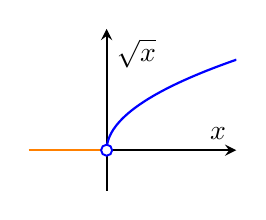
\begin{tikzpicture}
    \begin{axis}[
        width = 120,
        axis lines=middle,
        xlabel=$x$, ylabel=$\sqrt{x}$,
        samples=200,
        domain=-3:5,
        ymin=-1, ymax=3,
        xmin=-3, xmax=5,
        grid=both,
        thick, 
        xtick =\empty,
        ytick=\empty
    ]
    
    % Plot f(x) = 0 for x < 0
    \addplot[orange, thick, domain=-3:0] {0};
    
    % Plot f(x) = sqrt(x) for x > 0
    \addplot[blue, thick, domain=0:5] {sqrt(x)};
    
    % Open circle at (0,0) to indicate undefined
       \fill[color=white,draw=blue,line width=0.7pt] (axis cs:0,0) circle (2pt);
    
    \end{axis}
\end{tikzpicture}
